%%%%%%%%%%%%%%%%%%%%%%%%%%%%%%%%%%%%%%%%%
% Short Sectioned Assignment
% LaTeX Template
% Version 1.0 (5/5/12)
%
% This template has been downloaded from:
% http://www.LaTeXTemplates.com
%
% Original author:
% Frits Wenneker (http://www.howtotex.com)
%
% License:
% CC BY-NC-SA 3.0 (http://creativecommons.org/licenses/by-nc-sa/3.0/)
%
%%%%%%%%%%%%%%%%%%%%%%%%%%%%%%%%%%%%%%%%%

%----------------------------------------------------------------------------------------
%	PACKAGES AND OTHER DOCUMENT CONFIGURATIONS
%----------------------------------------------------------------------------------------

\documentclass[norsk]{article} % A4 paper and 11pt font size

\usepackage[T1]{fontenc} % Use 8-bit encoding that has 256 glyphs
\usepackage{fourier} % Use the Adobe Utopia font for the document - comment this line to return to the LaTeX default
\usepackage[english]{babel} % English language/hyphenation
\usepackage{amsmath,amsfonts,amsthm} % Math packages

% Added by Haavard %---------------------------------------------------------------------
\usepackage[utf8]{inputenc} % Norwegian letters
\usepackage{fullpage}
\usepackage{subcaption}
\usepackage[font={small, it}]{caption} % captions on figures and tables
\usepackage{graphicx}
\usepackage{color}
\usepackage{hyperref} % Use \autoref{ and \nameref{
\hypersetup{backref,
  colorlinks=true,
  breaklinks=true,
  %hidelinks, %uncomment to make links black
  linkcolor=blue,
  urlcolor=blue,
  citecolor=blue
}
\usepackage[all]{hypcap} % Makes hyperref jup to top of pictures and tables
% --------------------------------------------------------------------------------------

\usepackage{lipsum} % Used for inserting dummy 'Lorem ipsum' text into the template

\usepackage{sectsty} % Allows customizing section commands
\allsectionsfont{\centering \normalfont\scshape} % Make all sections centered, the default font and small caps

\usepackage{fancyhdr} % Custom headers and footers
\pagestyle{fancyplain} % Makes all pages in the document conform to the custom headers and footers
\fancyhead{} % No page header - if you want one, create it in the same way as the footers below
\fancyfoot[L]{} % Empty left footer
\fancyfoot[C]{} % Empty center footer
\fancyfoot[R]{\thepage} % Page numbering for right footer
\renewcommand{\headrulewidth}{0pt} % Remove header underlines
\renewcommand{\footrulewidth}{0pt} % Remove footer underlines
\setlength{\headheight}{13.6pt} % Customize the height of the header

\numberwithin{equation}{section} % Number equations within sections (i.e. 1.1, 1.2, 2.1, 2.2 instead of 1, 2, 3, 4)
\numberwithin{figure}{section} % Number figures within sections (i.e. 1.1, 1.2, 2.1, 2.2 instead of 1, 2, 3, 4)
\numberwithin{table}{section} % Number tables within sections (i.e. 1.1, 1.2, 2.1, 2.2 instead of 1, 2, 3, 4)

\setlength\parindent{0pt} % Removes all indentation from paragraphs - comment this line for an assignment with lots of text

%----------------------------------------------------------------------------------------
%	TITLE SECTION
%----------------------------------------------------------------------------------------

\newcommand{\horrule}[1]{\rule{\linewidth}{#1}} % Create horizontal rule command with 1 argument of height

\title{	
\normalfont \normalsize 
\textsc{NTNU} \\ [25pt] % Your university, school and/or department name(s)
\horrule{0.5pt} \\[0.4cm] % Thin top horizontal rule
\huge TMA4280 - project part 2\\ % The assignment title
\horrule{2pt} \\[0.5cm] % Thick bottom horizontal rule
}

\author{Håvard Kvamme, Jørgen Vågan, Magnus Aarskaug Rud} % Your name

\date{\normalsize\today} % Today's date or a custom date

\begin{document}

\maketitle % Print the title

%----------------------------------------------------------------------------------------
%	PROBLEM 1
%----------------------------------------------------------------------------------------
\abstract{In this project the Kongull cluster have been used to solve the homogenous 
					2D Poisson problem on the unit square, both Message sending and shared memory 
				  solution models have been implemented and compared.}

\section{Problem Description}

In this project the task is to solve the two-dimensional poisson problem as stated below.
\begin{align}
	-\nabla^2 u &= f  \text{ in } \Omega = (0,1)\times(0,1) \\
	u &=  0 \text{ on } \partial \Omega
\end{align}
%
The problem is solved using a fast diagonalization method. The derivation of the method can be found in \cite{poisson} ,
and the system of equation to be solved can be written as 
\begin{align}
	\underline{T} \; \underline{U} + 	\underline{U} \; \underline{T} = \underline{G} 	
	\label{eq:Matrix}
\end{align}
where $\underline{T}$ is the discrete second order partial differential operator in one direction, 
$\underline{G}$ is the discrete loading function multiplied with the steplength squared $h^2$ and $\underline{U}$ is the discrete solution
to the problem.
and the method can be summed up into the following three steps:


\begin{description}
	\item[step 1  -  $O(n^2\log(n))$] \hfill \\ \hfill \\
		Compute $\underline{\tilde{G}} = \underline{Q}^T\underline{G} \; \underline{Q} $    -    two matrix-matrix products 
		\hfill \\
   \item[step 2  -  $O(n^2)$] \hfill \\ \hfill \\ 
		Compute $\tilde{u}_{i,j} = \frac{\tilde{g}_{i,j}}{\lambda_i+\lambda_j}$    -    scalar addition and divition
		\hfill \\
	\item[step 3  -  $O(n^2log(n))$] \hfill \\ \hfill \\
		Compute $\underline{U} = \underline{Q}\underline{\tilde{U}} \; \underline{Q}^T $    -     two matrix-matrix products 
\end{description}

$\underline{Q}$ and $\underline{\Lambda}$ contains the eigenvectors and the eigenvalues of the discrete 
second order partial differential operator. 

Step 1 and 3 are solved using the infamous fast sine transform.

\section{Implementation strategy}
More detailled: Transposing - MPI - OpenMP

\section{Description of kongull cluster}
The Kongull cluster is a CentOS 5.3 linux cluster. It has 113 physical nodes, 
where 1 is used for login and 4 is used for I/O. The remaining 108 nodes are 
used for computing. The nodes are equipped with 2$\times$ 6-core 2.4 GHz processors, with 6$\times$ 512KiB 
(1 kibibyte = 1024 byte) L1-cache and a common 6 MiB (1 mebibyte = $1024^2$ bytes) L3-cache.
The compute nodes are spread out on 4 racks, 
(rack 0: 40 nodes, rack 2: 40 nodes, rack 1: 16 nodes; rack 3: 12 nodes) 
where the first 3 hold the HP AMP Opteron based nodes (2.4 GHz core speed) 
%\todo{clock speed?}
, while the last rack 
(rack 3) holds the new Dell intel based nodes (2$\times$ 2.60 GHz 8-core processors). In total 1344 compute nodes, with a ''Fat Tree'' network layout.
%\todo{is this okay? do i need a reference? https://www.hpc.ntnu.no/display/hpc/Kongull+Hardware }

% FAT TREE REF:  http://clusterdesign.org/fat-trees/
% KONGULL REF: http://clusterdesign.org/fat-trees/
%full name
%system
%type
%number of nodes
%a single node: details etc

%number of cores physical
%number of cores logical
%(logical cores = (physical cores)x(number of threads that can run through hyperthreading)
%(hyperthreading: For each physical core the OS addresses two virtual/logical cores and shares
%the workload between them when possible. The main function of hyperthreading is to increase 
%the number of independent instruction in the pipeline; it takes advantage of superscalar 
%architecture(inctruction level parallelism) in which multiple instructions operate
%on separate data in parallel.)
%CPU type
%theoretical total peak
%weight.

\section{Results}
%
\colorbox{yellow}{Need something about how this was run on Kongull?}\\
First it is important to verify that the code works correctly. This was done by comparing the results to an analytical solution and plotting the error for different problem sizes $n$. The problem chosen for this task was 
\begin{align}
  \label{eq:conv} 
  f = 5 \pi^2 \sin (\pi x) \sin (2 \pi y),
\end{align}
with the solution
\begin{align}
  u = \sin (\pi x) \sin (2 \pi y). 
\end{align}
The max norm was used to measure the error. The calculations were run with two threads on 1, 3 and 6 MPI processes, and the results can be found in Figure~\ref{fig:errVsn}. This plot is a log-log plot, with a reference line of slope $-2$. As the points follow the line, this means the method has quadratic converges. As the numerical scheme is a second order method, the figure confirms that our implementation is correct. For the rest of this section all tests are done with the $f$ in Eq.~\eqref{eq:conv}, unless specified otherwise.\\
%
\begin{figure}[h!]
\begin{center}
    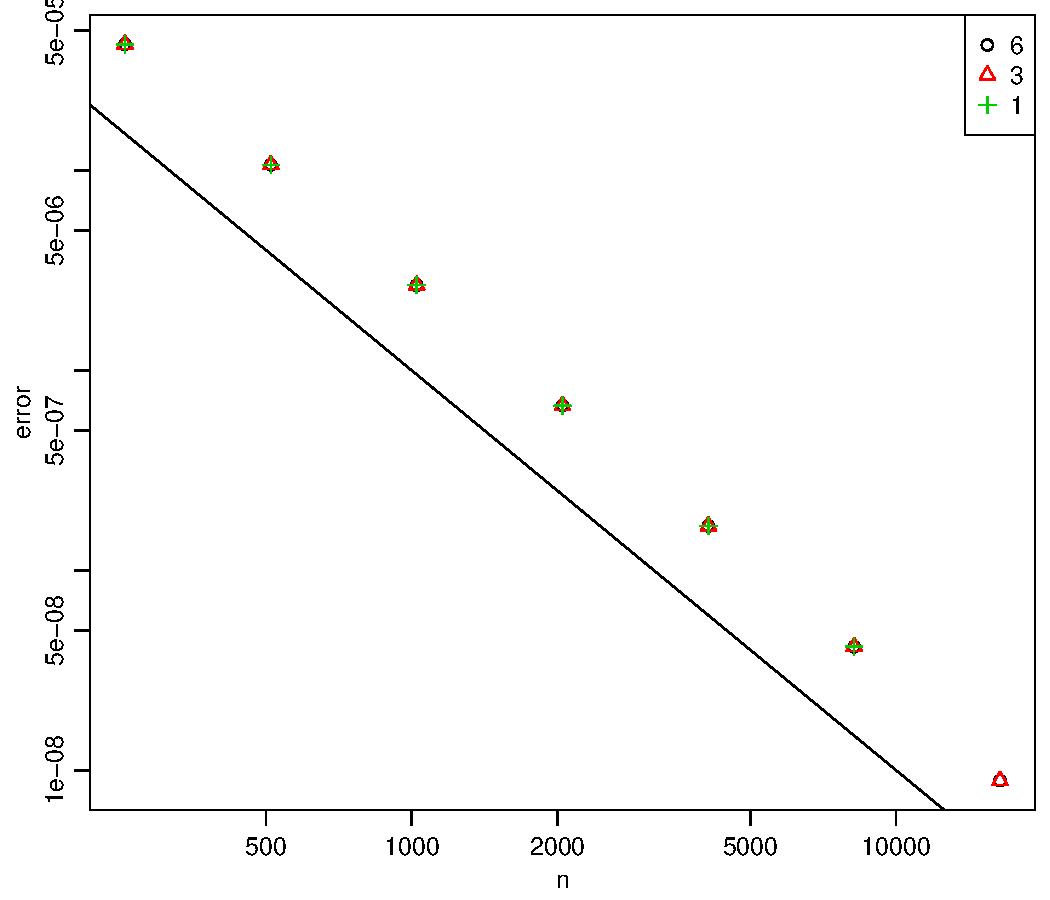
\includegraphics[scale=0.4]{./Figures/errVsn.pdf}
\end{center}
\caption{Loglog plot of the error as function of $n$. A reference line with slpe $-2$ is drawn. The problem in run on two threads with the number of processes specified in the legend.}
\label{fig:errVsn}
\end{figure}
%
\\
Next the problem was run on a single node where all 12 processors were utilized. The point was to investigate the performance of using threads versus MPI processes. Thus the relation between threads $t$ and processes $p$ is $p t = 12$ or $p = 12/t$. The calculations were done with $n = 2^{14} = 16384$. 
The same problem was repeated on three nodes where all 12 processors were utilized in the same way as above. The results can be found in Figure~\ref{fig:taskc}. Immediately it is clear there the times are pretty noisy. This is important to take into account later in the report, where the problem is only run once for each test case. It is clear from both plots that it is preferable to use only MPI processes and no openMP. 

While running only one MPI process and 12 threads on one node there is still some overhead from the MPI sending to itself and the work of reordering the data. Therefore the problem was solved on 12 threads without this overhead. The results are the red crosses in Figure~\ref{fig:taskc}. It is clear that it is a lot faster than with the MPI sending, but it is still slower than running with 12 MPI processes. 
\\
\begin{figure}[h!]
  \centering
  \begin{subfigure}[b]{0.48\textwidth}
    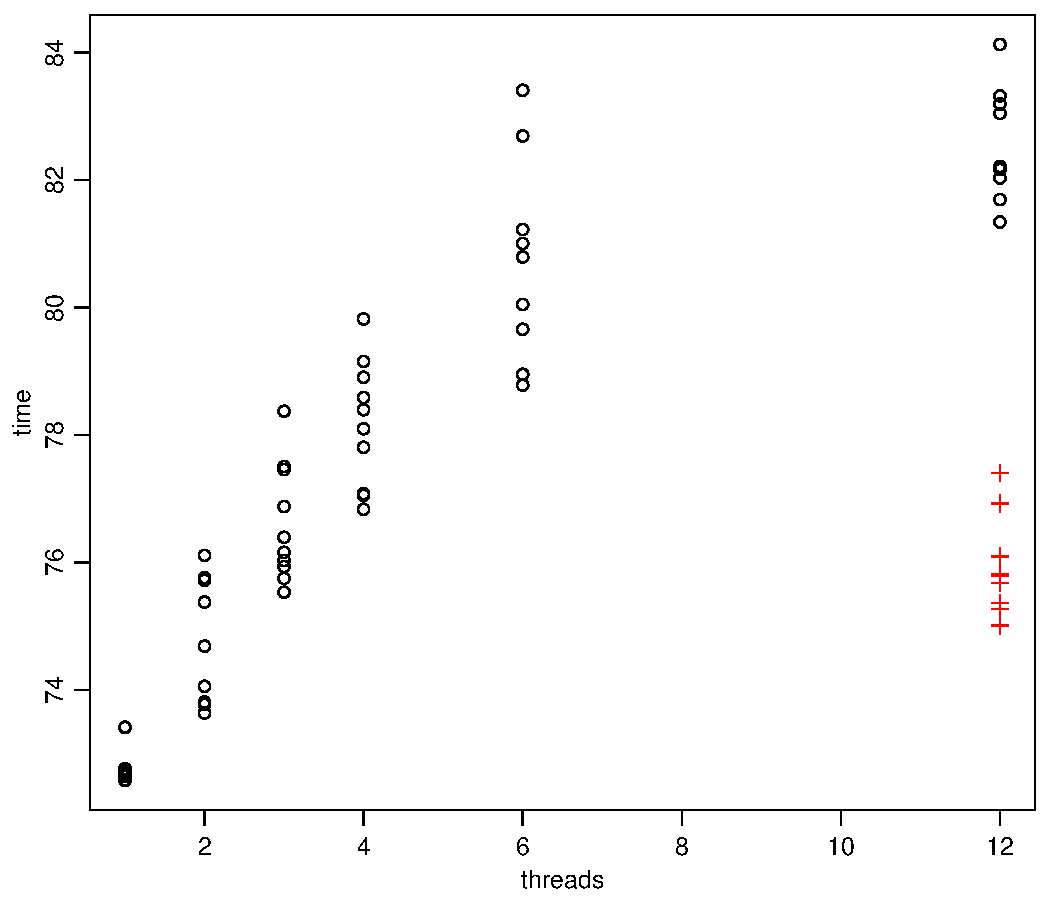
\includegraphics[width=\textwidth]{./Figures/taskc1.pdf}
  \end{subfigure}%
  \quad
  \begin{subfigure}[b]{0.48\textwidth}
    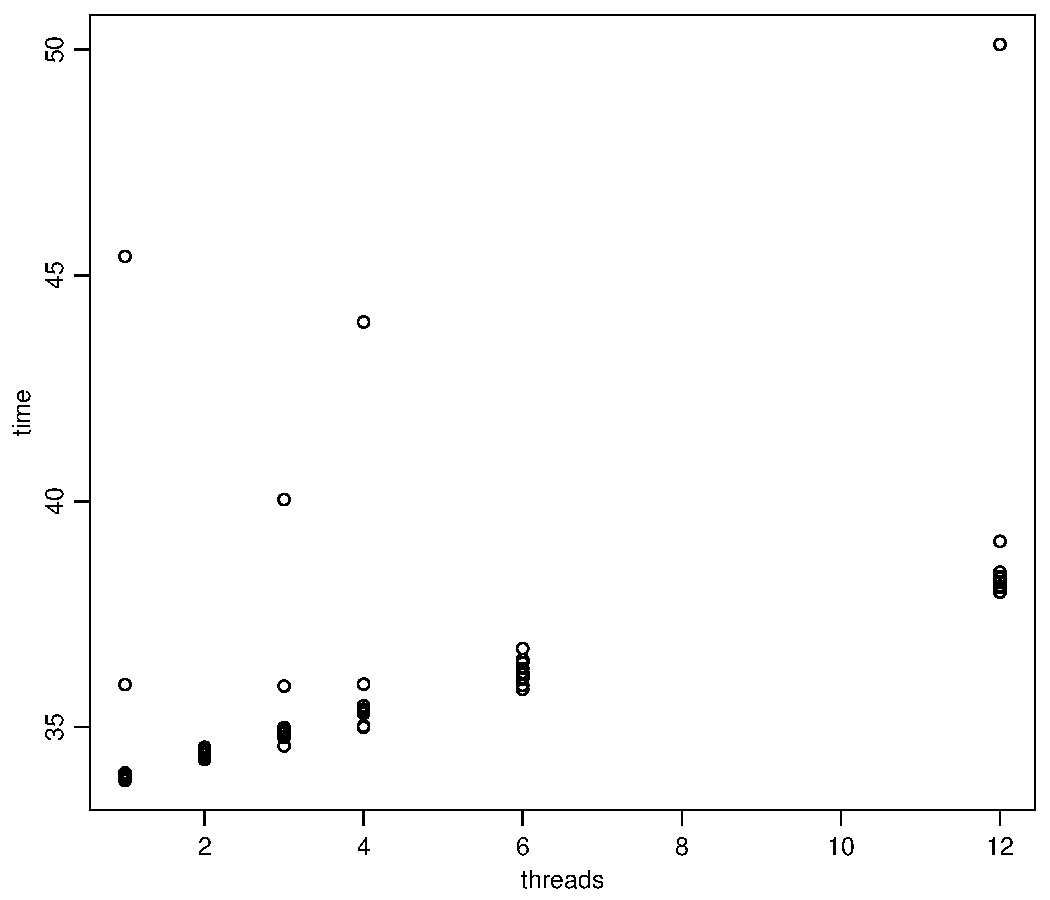
\includegraphics[width=\textwidth]{./Figures/taskc2.pdf}
  \end{subfigure}
          %(or a blank line to force the subfigure onto a new line)
  \vspace{1\baselineskip}
  \caption{Times (in seconds) for running MPI processes vs threads with $n = 2^{14}$. The total number of processors used are 12 per node, so the number of processes per node is 12 - threads. The left figure is run on one node, while the right is run on three nodes. The red crosses are run without any MPI sending at all.}
  \label{fig:taskc}
\end{figure}
\\
Next timing results were obtained by running the problem on different number of processes with one thread. Here up to three nodes were used, and a new node was only used if when there were no more free processors in the previous nodes. This was done for different problem sizes and plotted in Figure~\ref{fig:time1}. Sending between processes on a node should be faster than sending between nodes. This trend is clear in the figure, as the first points after utilizing an extra node (after the vertical lines), clearly do not follow the trend of the previous points. In Figure~\ref{fig:time2}, the same experiment is done, but with two treads instead of one. So here only up to 6 MPI processes were used on each node. Although it is clear from Figure~\ref{fig:taskc} that this should be worse than only using MPI processes, it is hard to distinguish Figure~\ref{fig:time1} and Figure~\ref{fig:time2}. To investigate how the time changed with only using threads on each node, the problem was run on 1 to 12 threads on 1 to three nodes. In Figure~\ref{fig:time3} this is plotted and we see the behavior is the same as in the other figures. It is reasonable to assume that for if run on more nodes, the time would eventually start to grow because of the overhead. There are some larger times at the end of Figure~\ref{fig:time1}, but this is probably just noise.\\
%
\begin{figure}[h!]
  \centering
  \begin{subfigure}[b]{0.48\textwidth}
    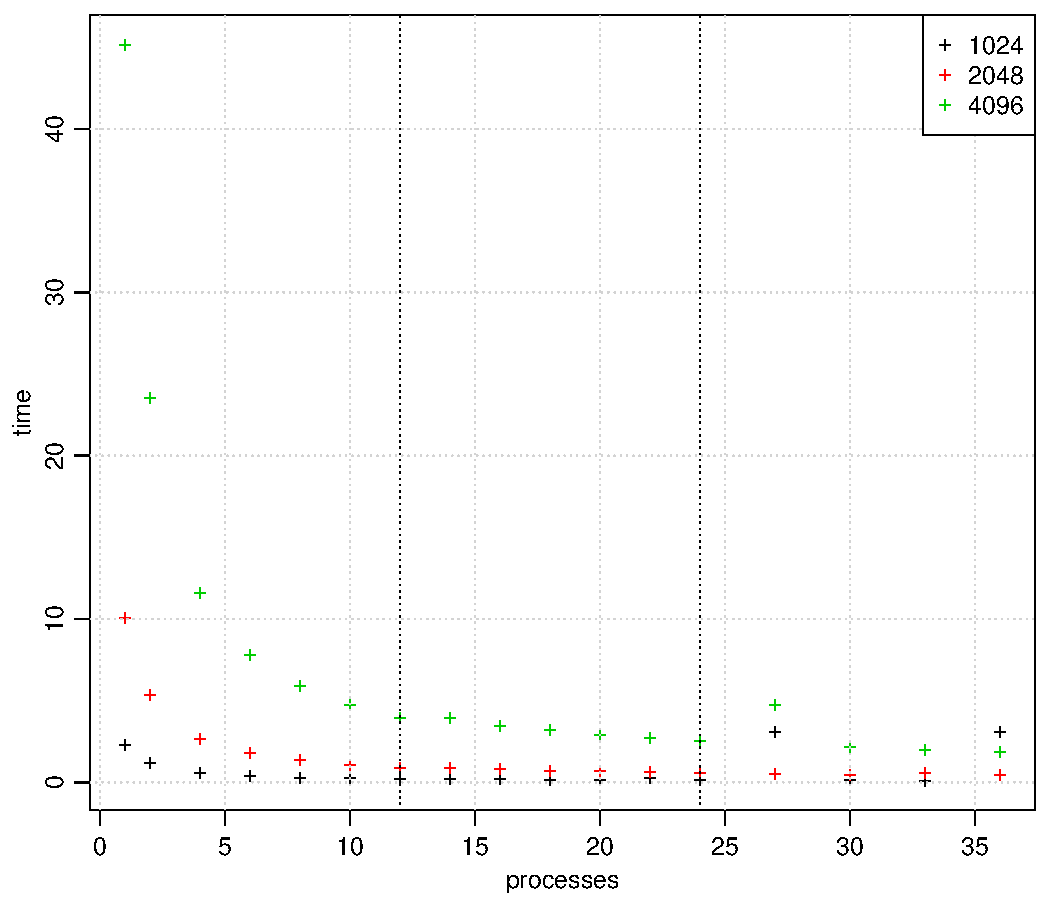
\includegraphics[width=\textwidth]{./Figures/taskbTimeProc1.pdf}
    \caption{}
    \label{fig:time1}
  \end{subfigure}%
  \quad
  \begin{subfigure}[b]{0.48\textwidth}
    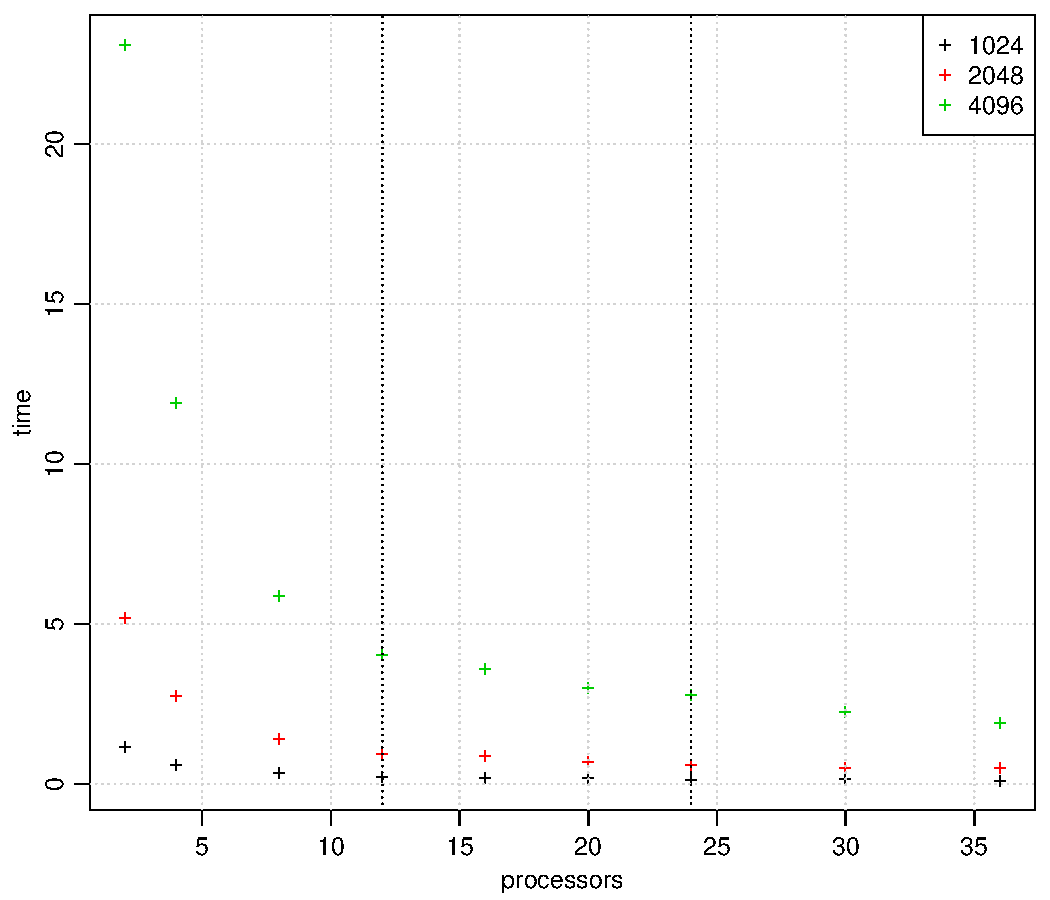
\includegraphics[width=\textwidth]{./Figures/taskbTimeProc2.pdf}
    \caption{}
    \label{fig:time2}
  \end{subfigure}
  \quad
  \begin{subfigure}[b]{0.48\textwidth}
    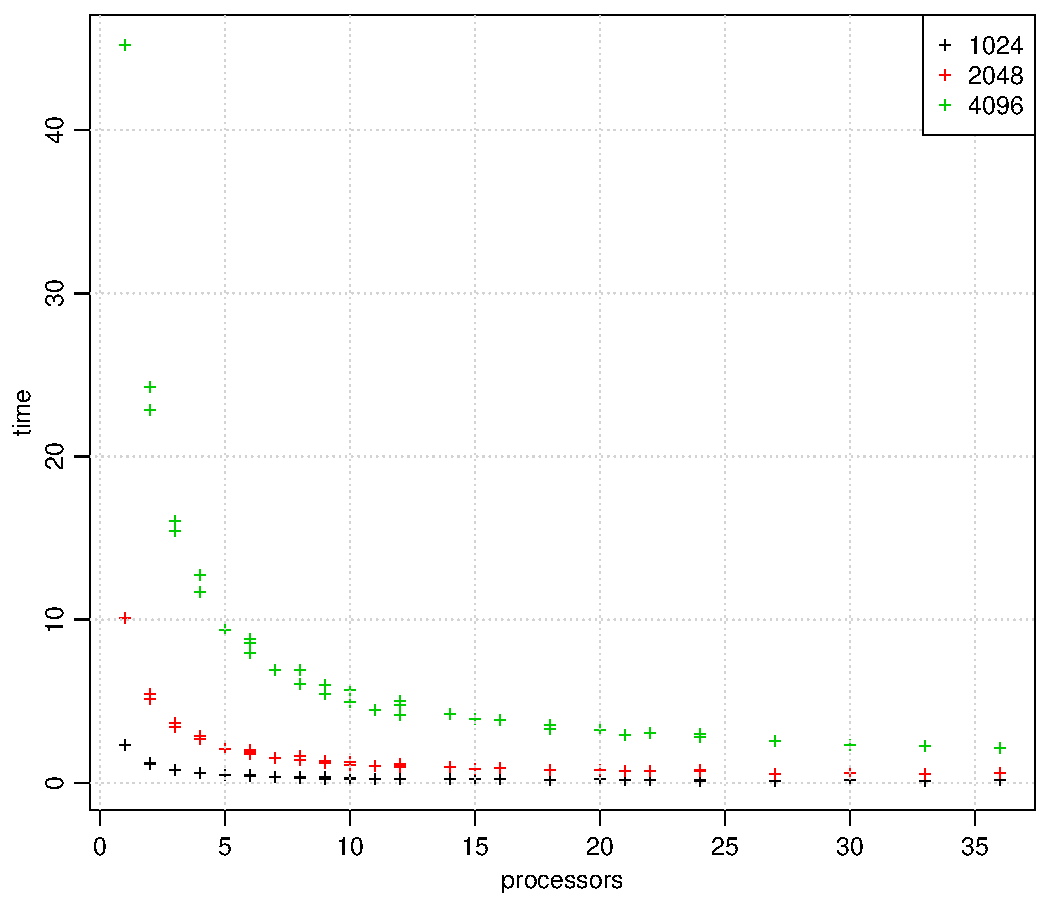
\includegraphics[width=\textwidth]{./Figures/taskbTimeNodesTimesThreads.pdf}
    \caption{}
    \label{fig:time3}
  \end{subfigure}
          %(or a blank line to force the subfigure onto a new line)
  \vspace{1\baselineskip}
  \caption{Times for running problem with different amount of processes. In the upper left figure each process has one thread, while in the upper right, each process has two treads. The problem is run on as few nodes as possible, and the processes are identically distributed among the nodes. The problem size $n$ is specified in the plots. The vertical lines separate the domain to show when 1, 2 and three nodes are used. In the bottom figure only one MPI process is run per node. Between 1 and 12 threads are run on each node.}
  \label{fig:Times}
\end{figure}
\\
While Figure~\ref{fig:Times} displays the times, it is hard see much from the plots. Another diagnostics tool is to plot the \textit{speedup} $t_1/t_i$, where $t_i$ is the time used by point $i$. If there is perfect speedup, i.e. for $i$ processes the time $t_i = t_1/i$, then the speedup should be a linear function of nr. of processes, with slope 1. The speedup, along with a reference line of slope 1, is plotted in Figure~\ref{fig:Speedup}.The setup is exacly the same as in Figure~\ref{fig:time}. Here it is clear that the speedup is better for larger problem sizes. This makes sense as the overhead becomes less significant as the time increases. Also note that there are some noisy points, especially for the smallest problem size. This was addressed in the beginning of this section. What is clear here is that the noise has a higher impact on small problems as the time is shorter, which makes perfect sense. Also here it is clear that there are more overhead when problem is done on one more node (see points after vertical lines in upper left figure). However, this is not the case for the red crosses. Whether this is noise of not is hard to say.\\
%
\begin{figure}[h!]
  \centering
  \begin{subfigure}[b]{0.48\textwidth}
    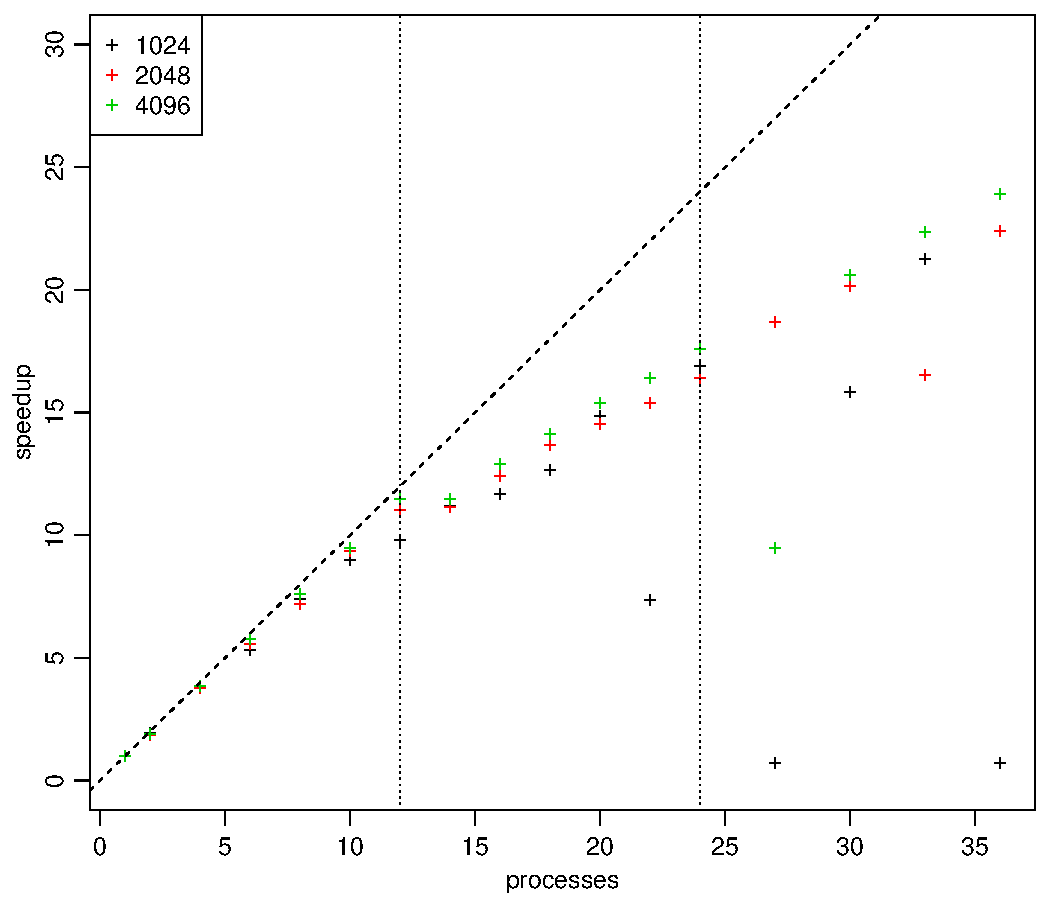
\includegraphics[width=\textwidth]{./Figures/taskbSpeedupProc1.pdf}
  \end{subfigure}%
  \quad
  \begin{subfigure}[b]{0.48\textwidth}
    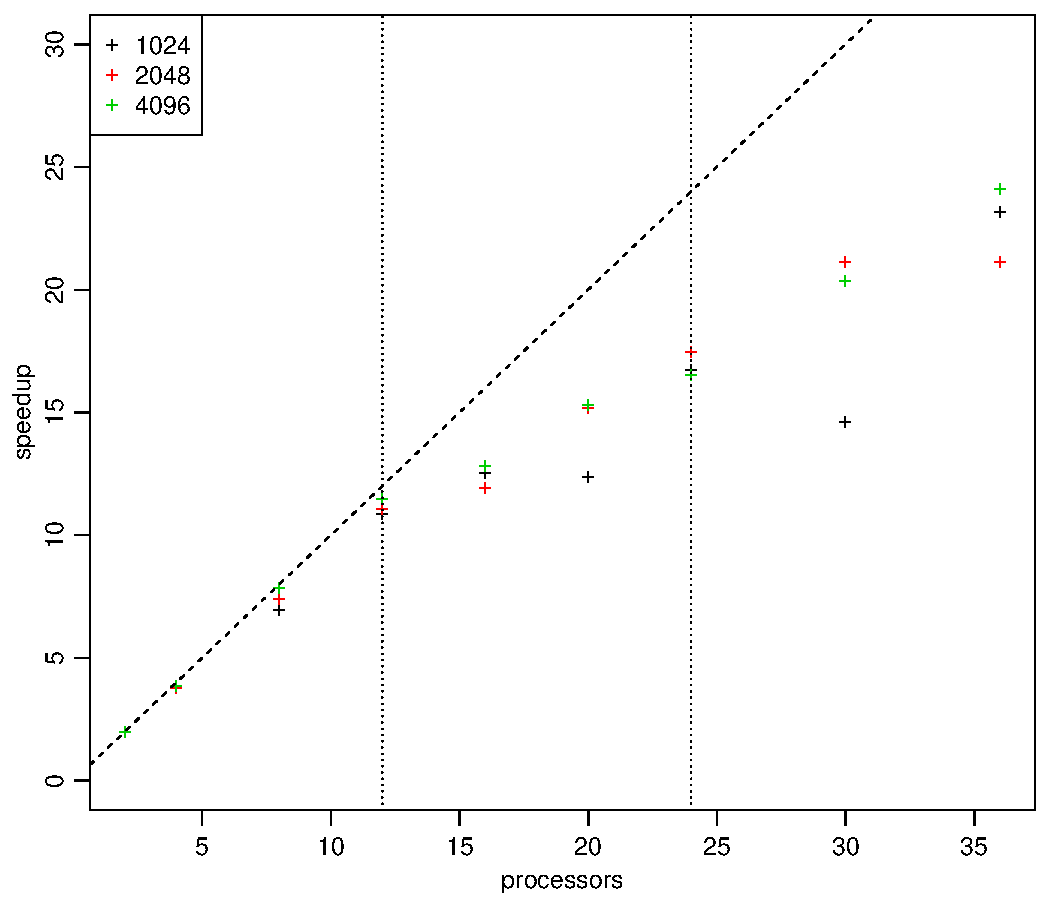
\includegraphics[width=\textwidth]{./Figures/taskbSpeedupProc2.pdf}
  \end{subfigure}
  \quad
  \begin{subfigure}[b]{0.48\textwidth}
    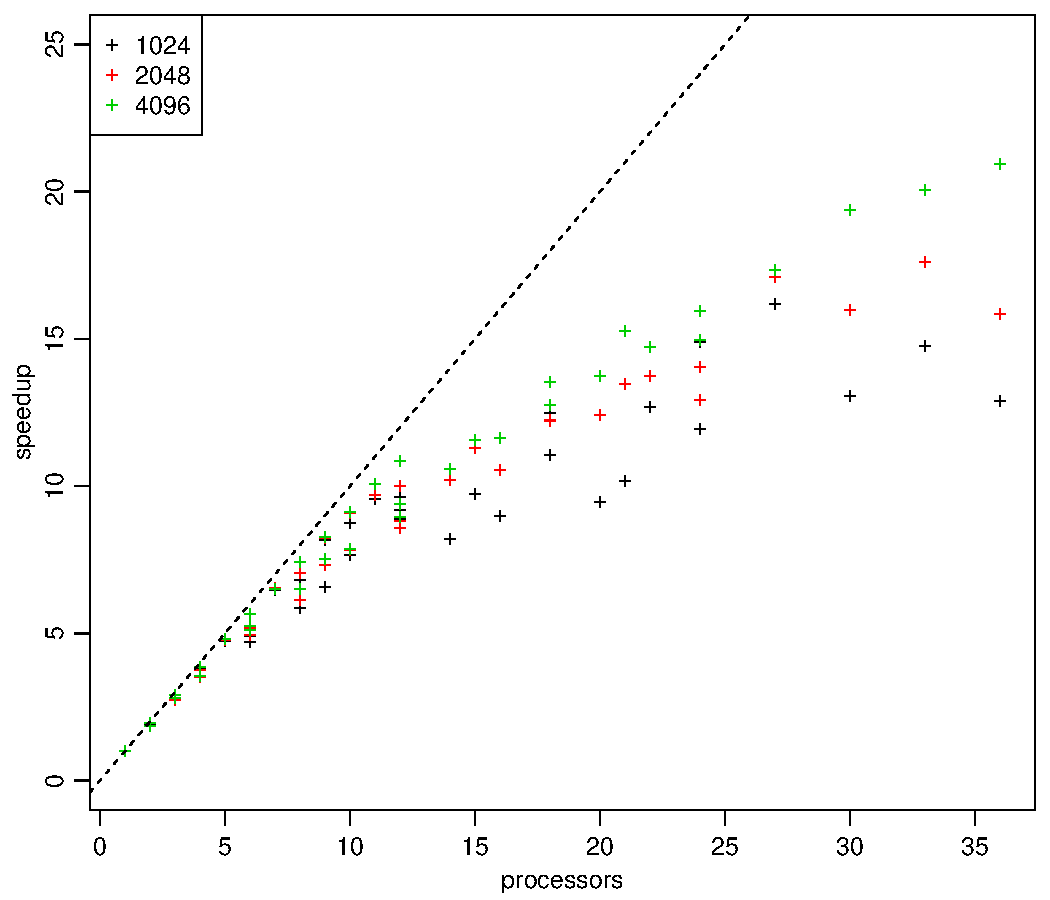
\includegraphics[width=\textwidth]{./Figures/taskbSpeedupNodesTimesThreads.pdf}
  \end{subfigure}
          %(or a blank line to force the subfigure onto a new line)
  \vspace{1\baselineskip}
  \caption{Speedup for running problem with different amount of processes. In the upper left figure each process has one thread, while in the upper right, each process has two treads. The problem is run on as few nodes as possible, and the processes are identically distributed among the nodes. There are drawn vertical lines to show when a new node is utilized, and a line with slope 1. The problem size $n$ is specified in the plots. In the bottom figure only one MPI process is run per node. Between 1 and 12 threads are run on each node.}
  \label{fig:Speedup}
\end{figure}
%
\\
Another diagnostics tool is to divide the speedup by number of processes. This is called the efficiency and is 1 if the speedup is perfect. This is shown in Figure~\ref{fig:Efficiency}. The plots show pretty much the same as Figure~\ref{fig:Speedup}, but the scale is different, so it is easier to see that there is no case of perfect speedup.
\\\colorbox{yellow}{Anything else to say here? Why do we need it?}
\\
\begin{figure}[h!]
  \centering
  \begin{subfigure}[b]{0.48\textwidth}
    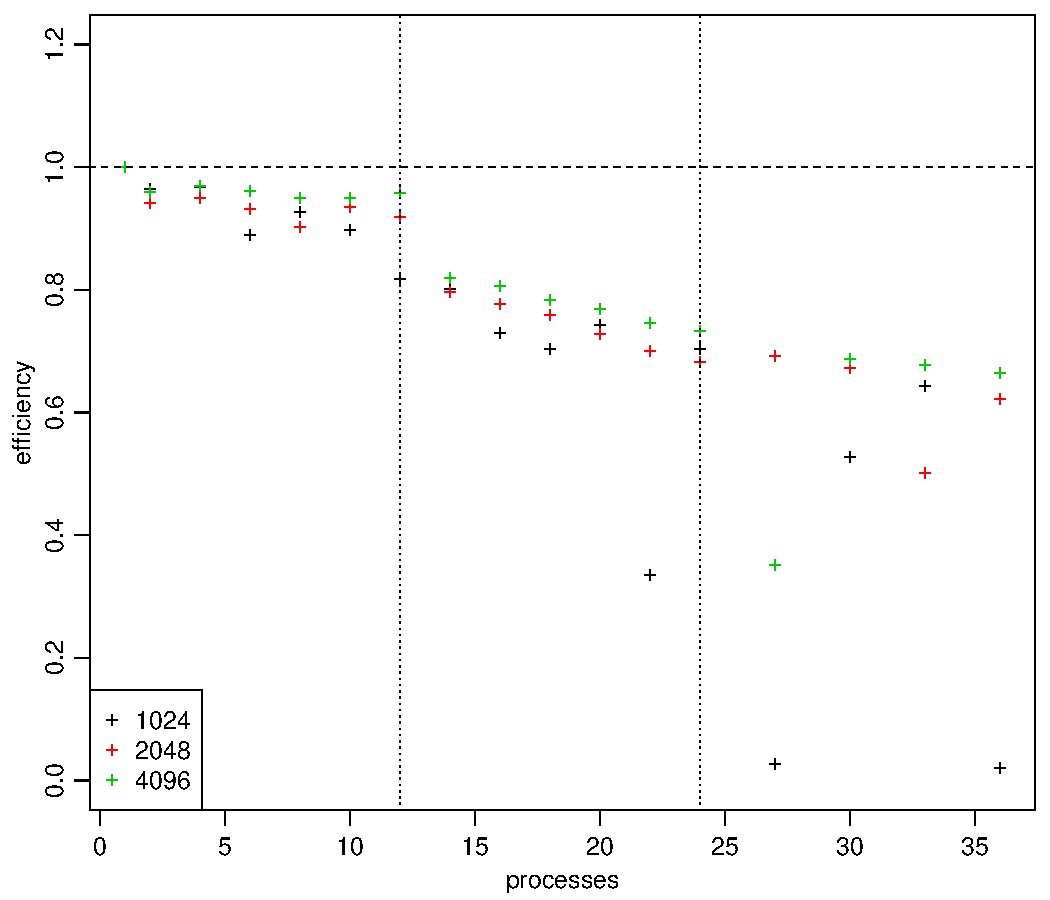
\includegraphics[width=\textwidth]{./Figures/taskbEfficiencyProc1.pdf}
  \end{subfigure}%
  \quad
  \begin{subfigure}[b]{0.48\textwidth}
    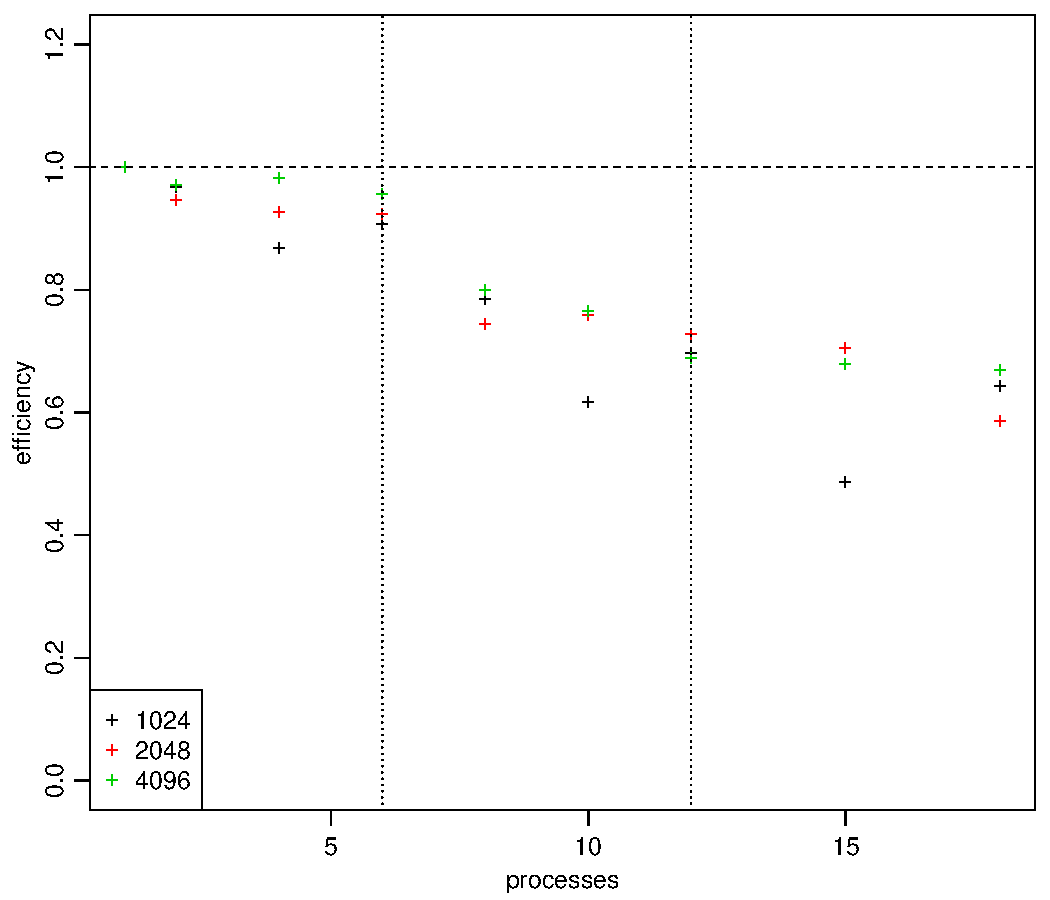
\includegraphics[width=\textwidth]{./Figures/taskbEfficiencyProc2.pdf}
  \end{subfigure}
          %(or a blank line to force the subfigure onto a new line)
  \vspace{1\baselineskip}
  \caption{Efficiency for running problem with different amount of processes. In the upper left figure each process has one thread, while in the upper right, each process has two treads. The problem is run on as few nodes as possible, and the processes are identically distributed among the nodes. There are drawn vertical lines to show when a new node is utilized, and a horizontal line at 1. The problem size $n$ is specified in the plots. In the bottom figure only one MPI process is run per node. Between 1 and 12 threads are run on each node.}
  \label{fig:Efficiency}
\end{figure}
%
\\
The time of the algorithm should be of order $O(n^2 \log(n)$. To investigate how the time scales with $n$, $time/n^2$ was plotted as a function of $n$. This is displayed in the left plot in Figure~\ref{fig:timeVsn}. The data used is the same as in Figure~\ref{fig:errVsn}. One can clearly see a upward trend for larger problem sizes. Therefore $time/(n^2 \log(n)$ was also plotted in Figure~\ref{fig:timeVsn}. Here the ratio looks like it is constant. So it seems like time is of order $O(n^2 \log(n)$. For small times, the overhead becomes significant, and that is probably why the first point is so much higher for 3 and 6 processes.
\begin{figure}[h!]
  \centering
  \begin{subfigure}[b]{0.48\textwidth}
    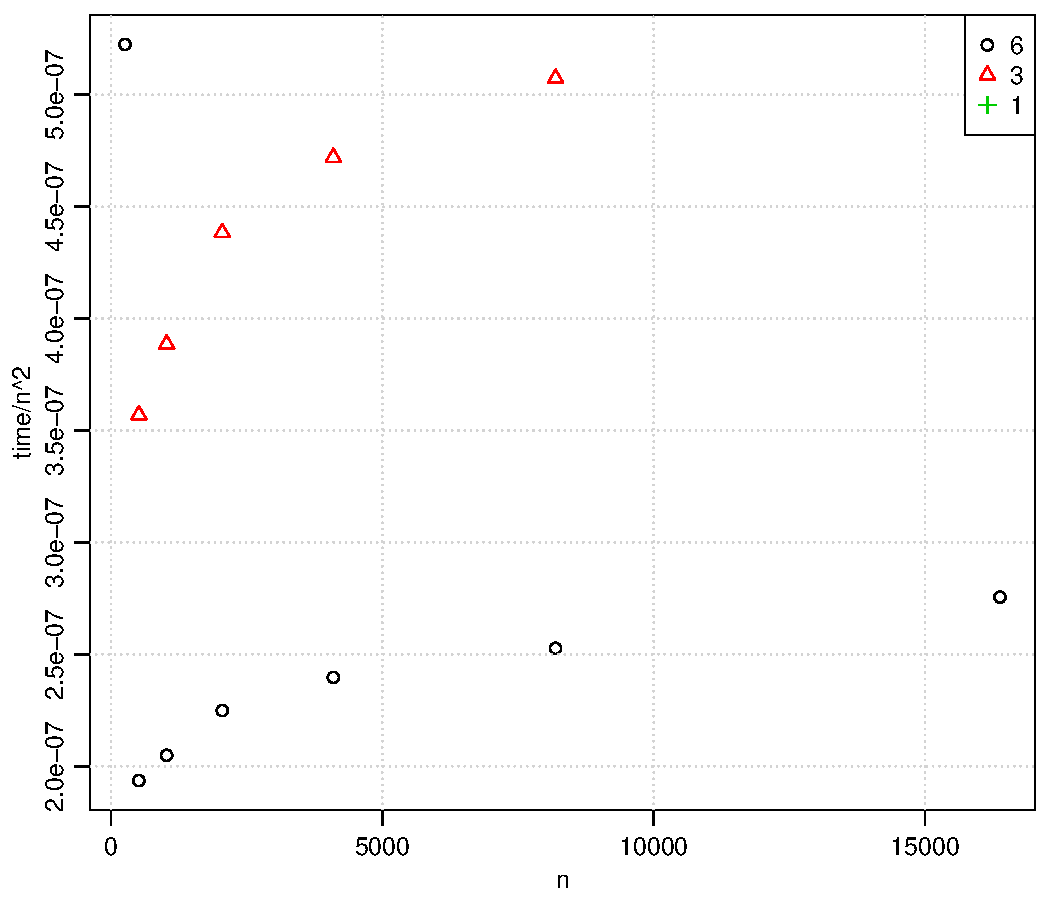
\includegraphics[width=\textwidth]{./Figures/timeOverN2Vsn.pdf}
  \end{subfigure}%
  \quad
  \begin{subfigure}[b]{0.48\textwidth}
    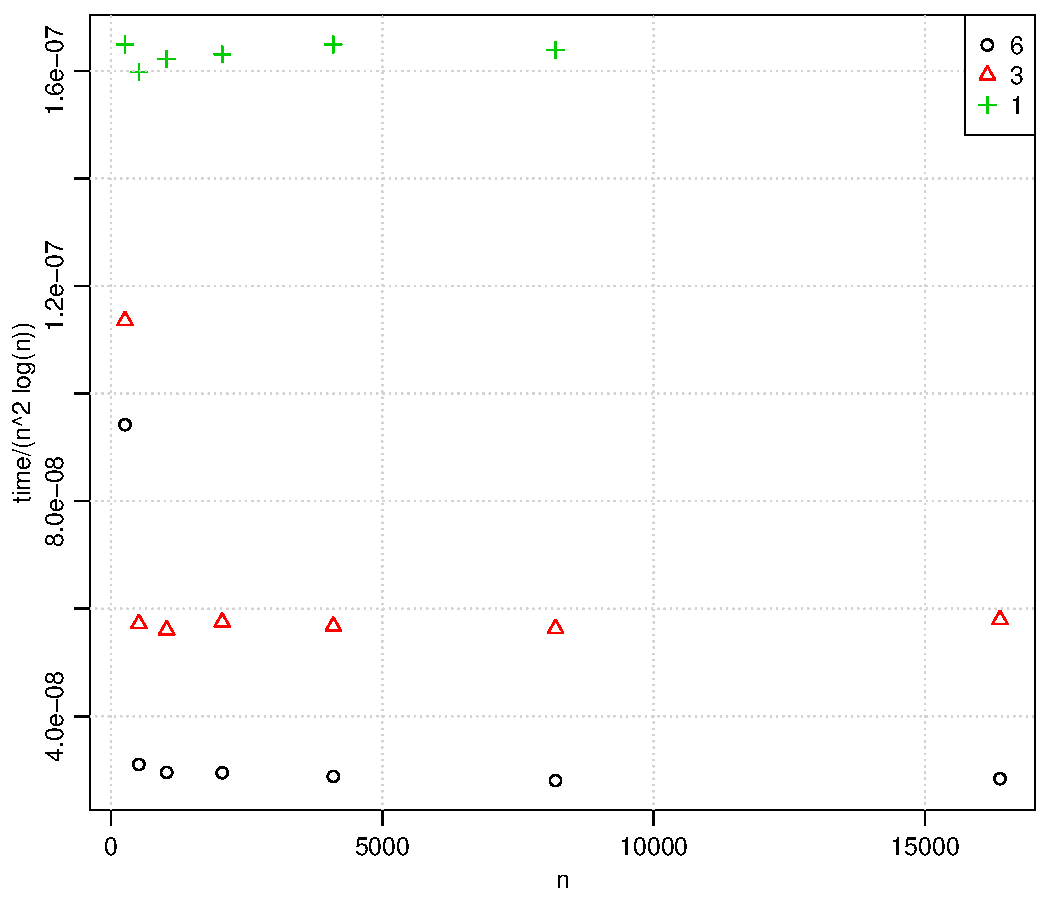
\includegraphics[width=\textwidth]{./Figures/timeOverN2LogNVsn.pdf}
  \end{subfigure}
          %(or a blank line to force the subfigure onto a new line)
  \vspace{1\baselineskip}
  \caption{Left plot is $Time/n^2$ as function of $n$. Illustrates how time scales with $n^2$. The right plot is $Time/(n^2 \log (n)$. The data is the same as in Figure~\ref{fig:errVsn}.}
  \label{fig:timeVsn}
\end{figure}

%\section{Analysis}

The time it will take to solve the problem with the implemented algorithm is of order $O(n^2\log(n))$.
Notice that as the problem size increases $\log(n)$ will be very small compared to $n^2$. It is therefore expected to see
the time increase almost as a function of $n^2$ for larger problem sizes.

The speedup $S_p$ of a program using $P$ processes is given as $S_p=\frac{T_1}{T_p}$. 
The theoretical upper bound of this value is the number and processes, and will often be much lower 
due to necessary serial code and sending costs. In the code used in this project the serial part of the parallelized program is 
very small, but the algorithm requires a lot of sending between processes. Since the kongull cluster is used one would expect 
that the sending cost will increase drastically when the program is runned on two or more nodes. It is therefore expected that 
the speedup between 12 and 14 processes will be very small since that is where kongull needs to use 2 nodes instead of just 1.

Another interesting and similar variable to study is the efficiency $\eta = \frac{S_p}{P}$, which has a theoretical upper bound 1.
The trend of this variable should be the same as the one observed in the speedup. 

SOME INFO ON THE LINEAR NETWORK MODEL! 

For larger problem sizes the overhead costs of creating and closing threads, sending procedures and general noise will have
a smaller effect on the total time. One can therefore expect that both the speedup and the efficiency will show a slightly better
trend for large problem sizes. 

OBSERVED RESULTS HERE ??

speedup calculations, theoretic and observed



\section{Discussion}

\subsection{Bottlenecks}

\subsection{The non-homogenous case}
If one were to solve the Poisson problem with non-homogenous boundary conditions ie. $u = g(x) $ on $\partial \Omega$, 
some minor modifications would have to be done. 
The matrix system that is generated through this algorithm does not include the effect of the boundary elements, 
and in practice this is the same as assuming that they are iqual zero. The second order differential operator on the elements 
closest to the boundary are on the form 
\begin{equation}
	-\frac{\partial^2 u_{i,j}}{\partial x^2} = -\frac{u_{i-1,j}-2u_{i,j}}{h^2}
\end{equation}
The incrementations of $i,j$ will depend on which boundary the element is close to, but the form of the operator is nevertheless the same.
The effect on equation REF MAIN MATRIX EQ is that the boundary element is added to the left side.
In the homogenous case this does not affect the numerical algorithm, but in the non-homogenous case the boundary value needs to be added to the 
right hand side as well. This is implemented before the FST is done and does not have any impact on the parallel implementation. 

\subsection{Variations in the loading function $f$}
The loading function simply needs to be evaluated in all the grid points and multiplied by the steplength, before the 
FST-procedure starts. The only thing that will differ from the serial code is the displacement each process have.

\subsection{Variations in the domain $\Omega$}
By defining the domain $\Omega = (0,L_x)\times(0,L_y)$ but keeping the same number of grid points in each direction 
the discretization of the laplacian operator would be changed. In the unit square the discrete laplacian is defined as 
\begin{equation}
	\Delta u_{i,j} = \frac{u_{i-1,j}-2u_{i,j}+u_{i+1,j}}{h^2}+\frac{u_{i,j-1}-2u_{i,j}+u_{i,j+1}}{h^2}.
\end{equation}
In the new domain the operator would be defined as  
\begin{equation}
	\Delta u_{i,j} = \frac{u_{i-1,j}-2u_{i,j}+u_{i+1,j}}{h_x^2}+\frac{u_{i,j-1}-2u_{i,j}+u_{i,j+1}}{h_y^2}.
\end{equation}
Where $h_x=L_x/n$ and $h_y=L_y/n$ defines the new steplengths in each direction. Notice that the infamous 5-point formula now takes quite a 
different form and some rewriting is necessary. 
The diagonalized matrix system will now end up looking as 
\begin{equation}
	\left( \frac{1}{h_x^2}\underline{T} \; \underline{U}+\frac{1}{h_y^2}\underline{U}\; \underline{T} \right) _{i,j}=f_{i,j}
\end{equation}

By continuing the diagonalization procedure st. $\underline{T}=\underline{Q}\;\underline{\Lambda}\;\underline{Q}^T $
and defining $\underline{\tilde{U}}= \underline{Q}^T\;\underline{U}\;\underline{Q}$ one is left with the matrix system 

\begin{equation}
	\frac{1}{h_x^2}\underline{\Lambda} \; \underline{\tilde{U}}+\frac{1}{h_y^2}\underline{\tilde{U}}\; \underline{\Lambda} =\underline{\tilde{F}}.
\end{equation}

Notice that the right hand side can not be initially multiplied with the steplength $h^2$ since the two terms on the left hand side
now have different coefficients. This has to be done in step 2 of the algorithm, and would be implemented in the following way; 

\begin{equation}
	\tilde{u}_{i,j} = \frac{\tilde{f}_{i,j}}{\lambda_i/h_x+\lambda_j/h_y}.
\end{equation}

The last part of the algorithm would not need any further changing.


\begin{thebibliography}{9}

		\bibitem{poisson}
		Einar M. Rønquist,
		\emph{The Poisson problem in $\mathbb{R}^2$: Diagonalization methods},
		Department of Mathematical Sciences,
		NTNU,N-7491 Trondheim, Norway,
		Revised by Arne Morten Kvarving, 2014.

\end{thebibliography}

\end{document}

